\sectionheading{5.24 ফ্লোচার্ট (Flowchart)}

কোনো Problem-এর Algorithm তৈরি করার পর ধাপগুলোকে শুধু লিখিতভাবে
না রেখে \textbf{নির্দিষ্ট প্রতীক ও প্রবাহরেখার সাহায্যে চিত্রে প্রকাশ}
করা যায়।

এতে কোন কাজের পর কোন কাজ হবে, কোথায় Decision নিতে হবে এবং
কাজের প্রবাহ কোন দিকে যাবে—তা এক নজরে বোঝা যায়।

%================================================
% Definition
%================================================

\booksubheading{Flowchart কাকে বলে?}

\begin{definitionbox}

\textbf{\color{darkTeal}সংজ্ঞা}

কোনো নির্দিষ্ট Problem সমাধানের প্রয়োজনীয় ধাপগুলোকে
\textbf{প্রচলিত প্রতীক (Symbol) ও প্রবাহরেখা (Flow line)-এর মাধ্যমে
চিত্রাকারে প্রকাশ করাকে Flowchart} বলে।

\end{definitionbox}

\textbf{সহজভাবে মনে রাখবে—}

\begin{center}

\textbf{Algorithm-এর ধাপ}
\(\longrightarrow\)
\textbf{Symbol দিয়ে চিত্র}
\(\longrightarrow\)
\textbf{Flowchart}

\end{center}

অর্থাৎ Algorithm ধাপগুলো লিখে দেয়, আর Flowchart সেই ধাপগুলোর
\textbf{চিত্রভিত্তিক প্রবাহ} দেখায়।

%================================================
% Importance
%================================================

\booksubheading{Flowchart কেন প্রয়োজন?}

Flowchart তৈরি করলে—

\begin{compacttwocolpoints}

\item Problem-এর Solution সহজে বোঝা যায়।

\item Program-এর কাজের ধারাবাহিকতা এক নজরে দেখা যায়।

\item Program লেখার আগে Logic যাচাই করা যায়।

\item ভুল বা অসংগতি শনাক্ত করা সহজ হয়।

\item Flowchart দেখে Program Code লেখা তুলনামূলক সহজ হয়।

\item Program ব্যাখ্যা, পরিবর্তন ও রক্ষণাবেক্ষণে সুবিধা হয়।

\end{compacttwocolpoints}

%================================================
% Types
%================================================

\booksubheading{Flowchart-এর প্রকারভেদ}

Flowchart প্রধানত দুই ধরনের—

\begin{enumerate}

\item
\textbf{Program Flowchart:}
কোনো নির্দিষ্ট Program-এর ধাপ, Calculation, Condition,
Decision ও Output-এর প্রবাহ চিত্রের মাধ্যমে প্রকাশ করে।

\item
\textbf{System Flowchart:}
কোনো সম্পূর্ণ System-এর Input, Processing, Storage ও Output-এর
পারস্পরিক সম্পর্ক ও তথ্যপ্রবাহ চিত্রের মাধ্যমে প্রকাশ করে।

\end{enumerate}

%================================================
% Symbols
%================================================

\booksubheading{Flowchart-এ ব্যবহৃত প্রধান প্রতীক}

\begin{tabularx}
{\linewidth}
{
|>{\centering\arraybackslash}p{0.22\linewidth}
|>{\RaggedRight\arraybackslash}p{0.27\linewidth}
|Y|
}

\hline

\rowcolor{softBlue}

\textbf{প্রতীক}
&
\multicolumn{1}{c|}{\textbf{নাম/অর্থ}}
&
\multicolumn{1}{c|}{\textbf{ব্যবহার}}

\\

\hline

%------------------------------------------------
% Process
%------------------------------------------------

\begin{tikzpicture}[baseline=(current bounding box.center)]

\node[
    fcProcess,
    minimum width=1.75cm,
    minimum height=5mm
]{};

\end{tikzpicture}

&
\textbf{প্রক্রিয়াকরণ (Process)}

&
Calculation বা Processing নির্দেশ করে।

\\

\hline

%------------------------------------------------
% Input / Output
%------------------------------------------------

\begin{tikzpicture}[baseline=(current bounding box.center)]

\node[
    fcIO,
    minimum width=1.75cm,
    minimum height=5mm
]{};

\end{tikzpicture}

&
\textbf{ইনপুট/আউটপুট}

&
Data গ্রহণ বা Result প্রদর্শন নির্দেশ করে।

\\

\hline

%------------------------------------------------
% Start / End
%------------------------------------------------

\begin{tikzpicture}[baseline=(current bounding box.center)]

\node[
    fcTerminal,
    minimum width=1.65cm,
    minimum height=5mm
]{};

\end{tikzpicture}

&
\textbf{শুরু/শেষ (Terminal)}

&
Flowchart-এর শুরু ও শেষ নির্দেশ করে।

\\

\hline

%------------------------------------------------
% Decision
%------------------------------------------------

\begin{tikzpicture}[baseline=(current bounding box.center)]

\node[
    fcDecision,
    minimum width=1.50cm,
    minimum height=6mm
]{};

\end{tikzpicture}

&
\textbf{সিদ্ধান্ত (Decision)}

&
Condition পরীক্ষা করে সিদ্ধান্ত গ্রহণ নির্দেশ করে।

\\

\hline

%------------------------------------------------
% Connector
%------------------------------------------------

\begin{tikzpicture}[baseline=(current bounding box.center)]

\node[
    fcConnector,
    minimum size=3.8mm
]{};

\end{tikzpicture}

&
\textbf{সংযোগ (Connector)}

&
Flowchart-এর বিচ্ছিন্ন অংশের মধ্যে সংযোগ স্থাপন করে।

\\

\hline

%------------------------------------------------
% Flow Direction
%------------------------------------------------

\begin{tikzpicture}[
    baseline=(current bounding box.center),
    >=Stealth
]

\draw[
    ->,
    line width=0.6pt
]
(0,0)--(0.55,0);

\draw[
    ->,
    line width=0.6pt
]
(0,0)--(-0.55,0);

\draw[
    ->,
    line width=0.6pt
]
(0,0)--(0,0.45);

\draw[
    ->,
    line width=0.6pt
]
(0,0)--(0,-0.45);

\end{tikzpicture}

&
\textbf{প্রবাহের দিক (Flow line)}

&
পরবর্তী ধাপে কাজের প্রবাহ কোন দিকে যাবে তা নির্দেশ করে।

\\

\hline

%------------------------------------------------
% Subroutine / Predefined Process
%------------------------------------------------

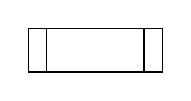
\begin{tikzpicture}[baseline=(current bounding box.center)]

\draw[
    line width=0.6pt
]
(0,0) rectangle (1.70,0.55);

\draw[
    line width=0.6pt
]
(0.23,0)--(0.23,0.55);

\draw[
    line width=0.6pt
]
(1.47,0)--(1.47,0.55);

\end{tikzpicture}

&
\textbf{সাবরুটিন / পূর্বনির্ধারিত প্রক্রিয়া}

&
Program-এর পূর্বনির্ধারিত অংশ বা Subroutine নির্দেশ করে।

\\

\hline

%------------------------------------------------
% Annotation
%------------------------------------------------

\begin{tikzpicture}[baseline=(current bounding box.center)]

\draw[
    line width=0.6pt
]
(-0.48,0)--(-0.12,0);

\draw[
    line width=0.6pt
]
(-0.12,-0.42)--(-0.12,0.42);

\draw[
    line width=0.6pt
]
(-0.12,0.42)--(0.72,0.42);

\draw[
    line width=0.6pt
]
(-0.12,-0.42)--(0.72,-0.42);

\end{tikzpicture}

&
\textbf{বর্ণনা/টীকা (Annotation)}

&
কোনো ধাপ বা কার্যক্রম সম্পর্কে প্রয়োজনীয় ব্যাখ্যা বা টীকা
দিতে ব্যবহৃত হয়।

\\

\hline

\end{tabularx}

%================================================
% MCQ Reminder
%================================================

\begin{rememberbox}

\textbf{\color{deepOrange}MCQ-তে বেশি গুরুত্বপূর্ণ}

\textbf{Start/End}
\(\rightarrow\)
Oval
\qquad
\textbf{Input/Output}
\(\rightarrow\)
Parallelogram

\textbf{Process}
\(\rightarrow\)
Rectangle
\qquad
\textbf{Decision}
\(\rightarrow\)
Diamond

\end{rememberbox}

%================================================
% Rules
%================================================

\booksubheading{Flowchart আঁকার সাধারণ নিয়ম}

Flowchart আঁকার সময়—

\begin{enumerate}

\item
প্রথমে \textbf{Start} এবং সর্বশেষে
\textbf{End/Stop} ব্যবহার করতে হয়।

\item
প্রতিটি কাজের জন্য নির্ধারিত উপযুক্ত Symbol ব্যবহার করতে হয়।

\item
Flow line বা Arrow দিয়ে কাজের প্রবাহের দিক দেখাতে হয়।

\item
সাধারণত Flow উপর থেকে নিচে অথবা বাম থেকে ডানে দেখানো হয়।

\item
Decision-এর শাখায় প্রয়োজন অনুযায়ী
\textbf{Yes/No} বা \textbf{True/False} লিখতে হয়।

\item
Flow line-এর অপ্রয়োজনীয় ছেদ এড়িয়ে চলতে হয়।

\item
প্রয়োজন হলে বিচ্ছিন্ন অংশ যুক্ত করতে
\textbf{Connector} ব্যবহার করতে হয়।

\item
Flowchart পরিষ্কার, সংক্ষিপ্ত ও যৌক্তিক হওয়া উচিত।

\end{enumerate}

%================================================
% General Structure
% Proper Flowchart symbols + connected arrows
%================================================

\textbf{সাধারণ কাঠামো—}

\begin{center}

\begin{tikzpicture}[node distance=4.5mm]

% Start
\node[
    fcTerminal,
    draw=darkBlue,
    fill=softBlue,
    minimum width=2.2cm
] (start)
{\textbf{Start}};

% Input
\node[
    fcIO,
    draw=mainTeal,
    fill=softGreen,
    minimum width=2.45cm,
    below=of start
] (input)
{\textbf{Input}};

% Process
\node[
    fcProcess,
    draw=darkBlue,
    fill=softBlue,
    minimum width=2.35cm,
    below=of input
] (process)
{\textbf{Process}};

% Output
\node[
    fcIO,
    draw=mainTeal,
    fill=softGreen,
    minimum width=2.45cm,
    below=of process
] (output)
{\textbf{Output}};

% End
\node[
    fcTerminal,
    draw=darkBlue,
    fill=softBlue,
    minimum width=2.2cm,
    below=of output
] (end)
{\textbf{End}};

% Connected Arrows
\draw[fcArrow]
(start.south)--(input.north);

\draw[fcArrow]
(input.south)--(process.north);

\draw[fcArrow]
(process.south)--(output.north);

\draw[fcArrow]
(output.south)--(end.north);

\end{tikzpicture}

\end{center}

%================================================
% Examples
%================================================

\booksubheading{Flowchart-এর উদাহরণ}

%================================================
% Example 1
%================================================

\begin{examplebox}{উদাহরণ–১: দুটি সংখ্যার যোগফল নির্ণয়}

\textbf{Problem:}
দুটি সংখ্যার যোগফল নির্ণয় করতে হবে।

\begin{center}

\begin{tikzpicture}[node distance=4.2mm]

\node[
    fcTerminal
] (s)
{Start};

\node[
    fcIO,
    below=of s
] (i)
{Input \textenglish{a, b}};

\node[
    fcProcess,
    below=of i
] (p)
{\textenglish{sum = a + b}};

\node[
    fcIO,
    below=of p
] (o)
{Print \textenglish{sum}};

\node[
    fcTerminal,
    below=of o
] (e)
{End};

\draw[fcArrow]
(s)--(i);

\draw[fcArrow]
(i)--(p);

\draw[fcArrow]
(p)--(o);

\draw[fcArrow]
(o)--(e);

\end{tikzpicture}

\end{center}

\textbf{সংক্ষেপে—}

\begin{center}

\textbf{Input a, b}
\(\longrightarrow\)
\textbf{sum = a + b}
\(\longrightarrow\)
\textbf{Print sum}

\end{center}

\end{examplebox}

%================================================
% Example 2
%================================================

\begin{examplebox}{উদাহরণ–২: ত্রিভুজের ক্ষেত্রফল নির্ণয়}

\textbf{Problem:}
ত্রিভুজের ভূমি ও উচ্চতা দেওয়া থাকলে ক্ষেত্রফল নির্ণয় করতে হবে।

\medskip

\textbf{Formula:}

\begin{center}

\textbf{
Area =
\(\frac{1}{2}\)
\(\times\)
ভূমি
\(\times\)
উচ্চতা
}

\end{center}

\begin{center}

\begin{tikzpicture}[node distance=4.2mm]

\node[
    fcTerminal
] (s)
{Start};

\node[
    fcIO,
    below=of s
] (i)
{Input \textenglish{b, h}};

\node[
    fcProcess,
    below=of i
] (p)
{\textenglish{Area = 1/2 * b * h}};

\node[
    fcIO,
    below=of p
] (o)
{Print \textenglish{Area}};

\node[
    fcTerminal,
    below=of o
] (e)
{End};

\draw[fcArrow]
(s)--(i);

\draw[fcArrow]
(i)--(p);

\draw[fcArrow]
(p)--(o);

\draw[fcArrow]
(o)--(e);

\end{tikzpicture}

\end{center}

\end{examplebox}

%================================================
% Example 3
%================================================

\begin{examplebox}{উদাহরণ–৩: একটি সংখ্যা জোড় না বিজোড় নির্ণয়}

\textbf{Problem:}
একটি সংখ্যা Even না Odd তা নির্ণয় করতে হবে।

\begin{center}

\begin{tikzpicture}[
    node distance=5mm and 18mm
]

\node[
    fcTerminal
] (s)
{Start};

\node[
    fcIO,
    below=of s
] (i)
{Input \textenglish{n}};

\node[
    fcDecision,
    below=6mm of i
] (d)
{\textenglish{n \% 2 = 0 ?}};

\node[
    fcIO,
    below left=9mm and 18mm of d
] (yes)
{Print ``Even''};

\node[
    fcIO,
    below right=9mm and 18mm of d
] (no)
{Print ``Odd''};

\coordinate[
    below=14mm of d
] (join);

\node[
    fcTerminal,
    below=5mm of join
] (e)
{End};

\draw[fcArrow]
(s)--(i);

\draw[fcArrow]
(i)--(d);

\draw[fcArrow]
(d.west)
-| node[pos=0.25,above]{Yes}
(yes.north);

\draw[fcArrow]
(d.east)
-| node[pos=0.25,above]{No}
(no.north);

\draw[fcArrow]
(yes.south)
|- (join);

\draw[fcArrow]
(no.south)
|- (join);

\draw[fcArrow]
(join)--(e);

\end{tikzpicture}

\end{center}

\textbf{মনে রাখবে:}

\textenglish{n \% 2 = 0}
হলে সংখ্যা \textbf{Even}, অন্যথায় \textbf{Odd}।

\end{examplebox}

%================================================
% Example 4
%================================================

\begin{examplebox}
{উদাহরণ–৪: একটি সংখ্যা ধনাত্মক, ঋণাত্মক নাকি শূন্য নির্ণয়}

\textbf{Problem:}
একটি সংখ্যা Positive, Negative নাকি Zero তা নির্ণয় করতে হবে।

\begin{center}

\begin{tikzpicture}[
    node distance=5mm and 18mm
]

\node[
    fcTerminal
] (s)
{Start};

\node[
    fcIO,
    below=of s
] (i)
{Input \textenglish{n}};

\node[
    fcDecision,
    below=6mm of i
] (d1)
{\textenglish{n > 0 ?}};

\node[
    fcIO,
    below left=9mm and 20mm of d1
] (pos)
{Print ``Positive''};

\node[
    fcDecision,
    below right=9mm and 18mm of d1
] (d2)
{\textenglish{n < 0 ?}};

\node[
    fcIO,
    below left=9mm and 15mm of d2
] (neg)
{Print ``Negative''};

\node[
    fcIO,
    below right=9mm and 15mm of d2
] (zero)
{Print ``Zero''};

\coordinate[
    below=18mm of d2
] (join);

\node[
    fcTerminal,
    below=5mm of join
] (e)
{End};

\draw[fcArrow]
(s)--(i);

\draw[fcArrow]
(i)--(d1);

\draw[fcArrow]
(d1.west)
-| node[pos=0.25,above]{Yes}
(pos.north);

\draw[fcArrow]
(d1.east)
-| node[pos=0.25,above]{No}
(d2.north);

\draw[fcArrow]
(d2.west)
-| node[pos=0.25,above]{Yes}
(neg.north);

\draw[fcArrow]
(d2.east)
-| node[pos=0.25,above]{No}
(zero.north);

\draw[fcArrow]
(pos.south)
|- (join);

\draw[fcArrow]
(neg.south)
|- (join);

\draw[fcArrow]
(zero.south)
|- (join);

\draw[fcArrow]
(join)--(e);

\end{tikzpicture}

\end{center}

\end{examplebox}

%================================================
% Basic Structure
%================================================

\booksubheading{Flowchart-এর মৌলিক গঠন (Basic Structure)}

Flowchart-এ সাধারণত নিচের মৌলিক গঠনগুলো ব্যবহার করা হয়—

\begin{tabularx}
{\linewidth}
{
|>{\bfseries}p{0.24\linewidth}
|Y
|Y|
}

\hline

\rowcolor{softBlue}

\multicolumn{1}{|c|}{\textbf{গঠন}}

&

\multicolumn{1}{c|}{\textbf{মূল ধারণা}}

&

\multicolumn{1}{c|}{\textbf{উদাহরণ}}

\\

\hline

Sequence

&

একটির পর একটি কাজ ধারাবাহিকভাবে সম্পন্ন হয়

&

যোগফল, ক্ষেত্রফল, Average

\\

\hline

Selection

&

কোনো Condition অনুযায়ী একটি পথ নির্বাচন করা হয়

&

Even/Odd, Positive/Negative

\\

\hline

Repetition বা Loop

&

একই কাজ কোনো শর্ত অনুযায়ী বারবার সম্পন্ন হয়

&

Series, পুনরাবৃত্তিমূলক Problem

\\

\hline

Jump

&

Flowchart-এর এক অংশ থেকে অন্য অংশে Control স্থানান্তর করা হয়

&

প্রয়োজন অনুযায়ী অন্য ধাপে যাওয়া

\\

\hline

\end{tabularx}

%================================================
% Characteristics
%================================================

\booksubheading{একটি ভালো Flowchart-এর বৈশিষ্ট্য}

একটি ভালো Flowchart—

\begin{compacttwocolpoints}

\item সহজ ও বোধগম্য হবে।

\item ধাপগুলো সঠিক ও যৌক্তিক ক্রমে থাকবে।

\item প্রতিটি কাজের জন্য সঠিক Symbol ব্যবহার করবে।

\item Flow-এর দিক স্পষ্ট থাকবে।

\item Decision-এর Branch পরিষ্কার থাকবে।

\item অপ্রয়োজনীয় Line crossing এড়িয়ে চলবে।

\item অপ্রয়োজনীয় Step থাকবে না।

\item Problem-এর সঠিক Solution প্রকাশ করবে।

\end{compacttwocolpoints}

%================================================
% Algorithm vs Flowchart
%================================================

\booksubheading{Algorithm ও Flowchart-এর পার্থক্য}

\begin{tabularx}
{\linewidth}
{
|>{\bfseries}p{0.20\linewidth}
|Y
|Y|
}

\hline

\rowcolor{softBlue}

\multicolumn{1}{|c|}{\textbf{বিষয়}}

&

\multicolumn{1}{c|}{\textbf{Algorithm}}

&

\multicolumn{1}{c|}{\textbf{Flowchart}}

\\

\hline

রূপ

&

Problem সমাধানের ধাপ লিখিতভাবে প্রকাশ করা হয়

&

Problem সমাধানের ধাপ চিত্রের মাধ্যমে প্রকাশ করা হয়

\\

\hline

প্রকাশ

&

সাধারণ ভাষা বা সহজ নির্দেশনা ব্যবহার করা যায়

&

নির্দিষ্ট Symbol ও Flow line ব্যবহার করা হয়

\\

\hline

তৈরি

&

তুলনামূলক সহজ ও দ্রুত

&

আঁকতে তুলনামূলক বেশি সময় লাগে

\\

\hline

বোঝা

&

বড় Problem-এ সম্পূর্ণ Flow এক নজরে বোঝা কঠিন হতে পারে

&

চিত্রের কারণে Flow সহজে বোঝা যায়

\\

\hline

পরিবর্তন

&

পরিবর্তন বা সংশোধন তুলনামূলক সহজ

&

বড় Flowchart পরিবর্তনে পুনরায় আঁকার প্রয়োজন হতে পারে

\\

\hline

\end{tabularx}

\begin{center}

\textbf{Algorithm = Solution-এর লিখিত পরিকল্পনা}

\vspace{0.5mm}

\textbf{Flowchart = সেই পরিকল্পনার চিত্রভিত্তিক প্রকাশ}

\end{center}

%================================================
% Common Mistakes
%================================================

\booksubheading{Flowchart আঁকার সময় সাধারণ ভুল}

\begin{compacttwocolpoints}

\item Start বা End symbol বাদ দেওয়া।

\item Input/Output-এর জন্য Rectangle ব্যবহার করা।

\item Process বা Decision-এর জন্য ভুল Symbol ব্যবহার করা।

\item Decision-এর Yes/No Branch না দেখানো।

\item Arrow-এর Direction না দেওয়া।

\item Flow line অপ্রয়োজনে Cross করা।

\item প্রয়োজন হলেও Connector ব্যবহার না করা।

\item Flowchart অপ্রয়োজনীয়ভাবে জটিল করা।

\end{compacttwocolpoints}

%================================================
% Final Reminder
%================================================

\begin{rememberbox}

\textbf{\color{deepOrange}মনে রাখবে}

\begin{itemize}

\item
\textbf{Flowchart} হলো Problem সমাধানের ধাপগুলোর
\textbf{চিত্রভিত্তিক প্রকাশ}।

\item
\textbf{Oval}
\(\rightarrow\)
Start/End।

\item
\textbf{Parallelogram}
\(\rightarrow\)
Input/Output।

\item
\textbf{Rectangle}
\(\rightarrow\)
Process।

\item
\textbf{Diamond}
\(\rightarrow\)
Decision।

\item
\textbf{Arrow}
\(\rightarrow\)
Flow-এর দিক।

\item
\textbf{Connector}
\(\rightarrow\)
বিচ্ছিন্ন অংশ যুক্ত করে।

\item
Flowchart-এর মৌলিক গঠন—
\textbf{Sequence, Selection, Repetition/Loop ও Jump}।

\item
Decision থেকে সাধারণত
\textbf{Yes/No}
বা
\textbf{True/False}
Branch বের হয়।

\item
Flowchart-এর ধাপগুলো
\textbf{পরিষ্কার, সংক্ষিপ্ত ও যৌক্তিক} হওয়া উচিত।

\item
দ্রুত মনে রাখবে—

\begin{center}

\textbf{Problem বুঝি}
\(\longrightarrow\)
\textbf{Algorithm লিখি}
\(\longrightarrow\)
\textbf{Flowchart আঁকি}
\(\longrightarrow\)
\textbf{Code করি}

\end{center}

\end{itemize}

\end{rememberbox}

\small

%================================================
% 5.25 Python Introduction
%================================================

